\chapter{Simulador de radiología diagnóstica} 
\label{cap:xray}

Se denomina proyecciones radiológicas al procedimiento de situar tanto al paciente como el equipo de radiología para conseguir una imagen de una parte concreta de la anatomía del paciente. Estas proyecciones son la forma más habitual de hacer un diagnóstico por imagen médica, en concreto, utilizando la tecnología de rayos X. Esta técnica define una proyección por cada parte del cuerpo, y requiere por cada procedimiento una postura del paciente y configuración del equipo de radiografía concreto. 

En este capítulo se va a mostrar otro ejemplo una herramienta que proporcione un caso de uso real para el algoritmo propuesto en esta tesis. Será posible incorporar la técnica de posicionamiento de un paciente virtual con el objetivo de proporcionar al usuario cualquier postura necesaria. De esta manera, el usuario podrá entrenar las habilidades necesarias requeridas para el procedimiento médico.
El método propuesto proporciona deformaciones realistas en tiempos interactivos que permiten generar un entorno de entrenamiento para los usuarios.
%Comentar cosas de aprendizaje por la cual necesitamos un simulador

Por tanto, un simulador de \ac{RV} puede ayudar a mejorar el proceso de aprendizaje de los estudiantes de radiología. Las herramientas de \ac{RV} permiten entrenar procedimientos médicos en un entorno seguro. Sobre todo, esto se vuelve especialmente importante si el entorno de trabajo no es seguro ni para pacientes ni para los propios profesionales, evitando en este caso radiaciones peligrosas para la salud. Sin necesidad de pacientes reales, y sin límites de tiempo, un simulador de radiología diagnóstica proporciona una herramienta útil para practicar.

Como ha sido introducido anteriormente en la sección \ref{art:xraysim}, existen métodos de aprendizaje para ayudar al estudiante de radiología, pero se han encontrado las siguientes limitaciones en el proceso:

\begin{itemize}
\item Principalmente, los profesores usan repetidamente las mismas imágenes estáticas en sus clases, presentando el mismo caso una y otra vez.
\item No se pueden conseguir nuevas imágenes médicas instantáneamente para las clases.
\item No es posible variar la configuración de la anatomía mostrada ni conseguir diferentes anatomías para una misma configuración.
\item ProjectionVR$^{TM}$ es un buen simulador para enseñar las técnicas de diagnóstico por imagen, pero sus ejemplos son limitados a las imágenes y anatomías estáticas incluidas en el software.
\end{itemize}

Con estas limitaciones, en este capítulo se ha propuesto crear un simulador de radiología diagnóstica que pueda suplir las carencias antes citadas. En esta herramienta, estudiantes y profesores serán capaces de revisar numerosos de casos diferentes, con la posibilidad de probar infinidad de configuraciones de la máquina de rayos X incluso pudiendo trabajar con ejemplos incorrectos que no son habitualmente mostrados.


La idea de construir un simulador de \ac{RV} surge como colaboración entre el autor de esta tesis y un miembro del proyecto \ac{RASimAs}. Por un lado, se proporciona la capacidad de generar variabilidad anatómica, utilizando el algoritmo propuesto en esta tesis como técnica que permite modificar la anatomía del paciente con la finalidad de mover al paciente a su posición final.
Por otra parte, \emph{Franck P. Vidal} de la \emph{Universidad de Bangor}, dirige el proyecto \emph{gVirtualXray}\cite{vidal2009simulation} que permite simular imágenes generadas por Rayos X en entornos clínicos. La unión de estos dos métodos permitirá crear un simulador que contribuya a mejorar el entrenamiento de radiólogos noveles en el diagnóstico por imagen médica de forma interactiva y segura.


\section{gVirtualXray}
\label{xray:context}
Una de las principales características de la librería \emph{gVirtualXray} es la capacidad de simular imágenes realistas de rayos X en tiempo real. La interacción es una cualidad fundamental en cualquier simulador de \ac{RV}, por lo que esta librería es perfecta para la creación de una aplicación de diagnóstico por imagen. 
\emph{gVirtualXray} implementa la ley de \emph{Beer-Lambert} utilizando la arquitectura de las tarjetas gráficas que permiten calcular el recorrido del rayo X simulado, en vez de utilizar una simulación de Monte Carlo más habitual en la bibliografía \cite{vidal2009simulation}. La fidelidad de las imágenes producidas (Fig. \ref{fig:validation}) por esta librería se han validado usando \emph{Geant4}, una herramienta desarrollada por el \emph{CERN} que se encuentra como referencia en el estado del arte de la simulación de rayos X.

\begin{figure}[h]
    \begin{subfigure}[b]{0.25\linewidth}
        \centering
        {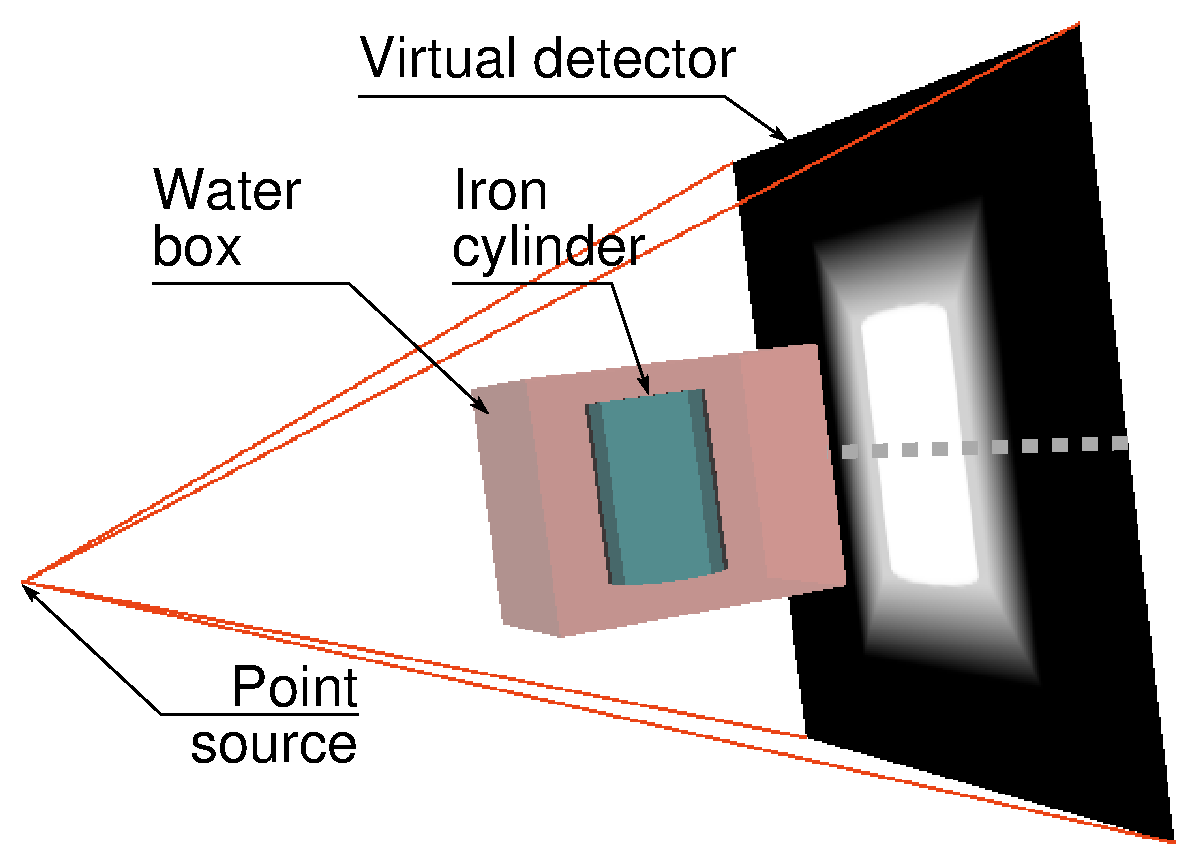
\includegraphics[width=0.8\linewidth]{IMG/figure3a.eps}}
        \caption{\label{subfig:polychromatismA} Escena de prueba.}
    \end{subfigure}
    \null\hfill
     \begin{subfigure}[b]{0.25\linewidth}
        \centering
        {\includegraphics[width=\linewidth]{IMG/figure6a.eps}}
        \caption{\label{subfig:GPU} Imagen determinista simulada  usando \emph{gVirtualXRay}.}
    \end{subfigure}
    \null\hfill
    \begin{subfigure}[b]{0.25\linewidth}
        \centering
        {\includegraphics[width=\linewidth]{IMG/figure6b.eps}}
        \caption{\label{subfig:Gate} Imagen simulada utilizando \emph{Monte Carlo} en \emph{Geant4}.}
    \end{subfigure}

\caption{\label{fig:validation} Ejemplo de la evaluación para la herramienta \emph{gVirtualXRay}.}
\end{figure}


El uso de la ley de atenuación (\emph{Beer-Lambert}) permite la posibilidad de simular eficientemente las imágenes de rayos X de cualquier superficie poligonal utilizando la arquitectura de las tarjetas gráficas, \emph{OpenGL} y \ac{GLSL}. La ecuación \emph{Beer-Lambert} se resuelve para cada punto de la imagen simulada, donde esta ley relaciona la absorción de la luz (en este caso fotones) con las propiedades del material por el cual la luz está atravesando. Esto da como resultado la posibilidad de generar imágenes visualmente realistas de radiografías y fluoroscópicas. 
La simulación está definida por varios parámetros donde lo más importantes tanto el emisor y el detector de rayos X como los objetos que serán virtualmente irradiados. 
\begin{itemize}
    \item Emisor: Simula la forma que tendría la fuente de fotones de una maquina de rayos X. Permite simular el emisor como si fuera un punto, una línea, un cubo o un conjunto de puntos. Además, se puede configurar su espectro de emisión a través de una lista discreta de protones que tienen la misma o diferentes energías.
    \item Detector: Define un plano que se traduce en el número de \emph{píxeles} que tendrá la imagen final, además de definir el número de rayos que simulará la librería. Normalmente, este plano se encuentra perpendicular a la dirección de los rayos, pero no es necesario.
    \item Modelos superficiales: mallados poligonales que tienen unas propiedades físicas. Estas propiedades se pueden definir a través de su composición química (porcentaje de átomos de determinado elemento químico)  o por su radio-densidad definida por la escala \emph{Hounsfield}. Esta escala es más habitual en entornos médicos. La conversión entre las dos definiciones es posible gracias a \cite{Schneider2000}.
\end{itemize}

Las propiedades físicas de las mallas superficiales son usadas para calcular los coeficientes que se usarán en la ley de atenuación para cada espectro del haz incidente. La correspondencia entre ellos se puede consultar en la base de datos \emph{XCOM} creada por \emph{National Institute of Standards
and Technology (NIST)}\cite{XCOM}






